% respuesta1.tex

Al correr el programa, que calcula el método de diferencias divididas de newton para interpolar la función:
\begin{equation*}
	f(x) = \frac{1}{1 + (\frac{5x}{10})^2}
\end{equation*}
En el intervalo de $[-10, 10]$, con 5, 8 y 11 nodos igualmente espaciados, se obtuvieron los siguientes coeficientes:

Para $n = 4$ se obtiene el siguiente polinomio:
\begin{dmath}
P_0(x) = 0.03846154 +0.01989390 * (x +10.00000000 ) +0.01525199 * (x +10.00000000 ) * (x +5.00000000 ) -0.00331565 * (x +10.00000000 ) * (x +5.00000000 ) * (x -0.00000000 ) +0.00033156 * (x +10.00000000 ) * (x +5.00000000 ) * (x -0.00000000 ) * (x -5.00000000 )
\end{dmath}
La grafica de $P_0(x)$:
\begin{figure}[H]
	\centering
	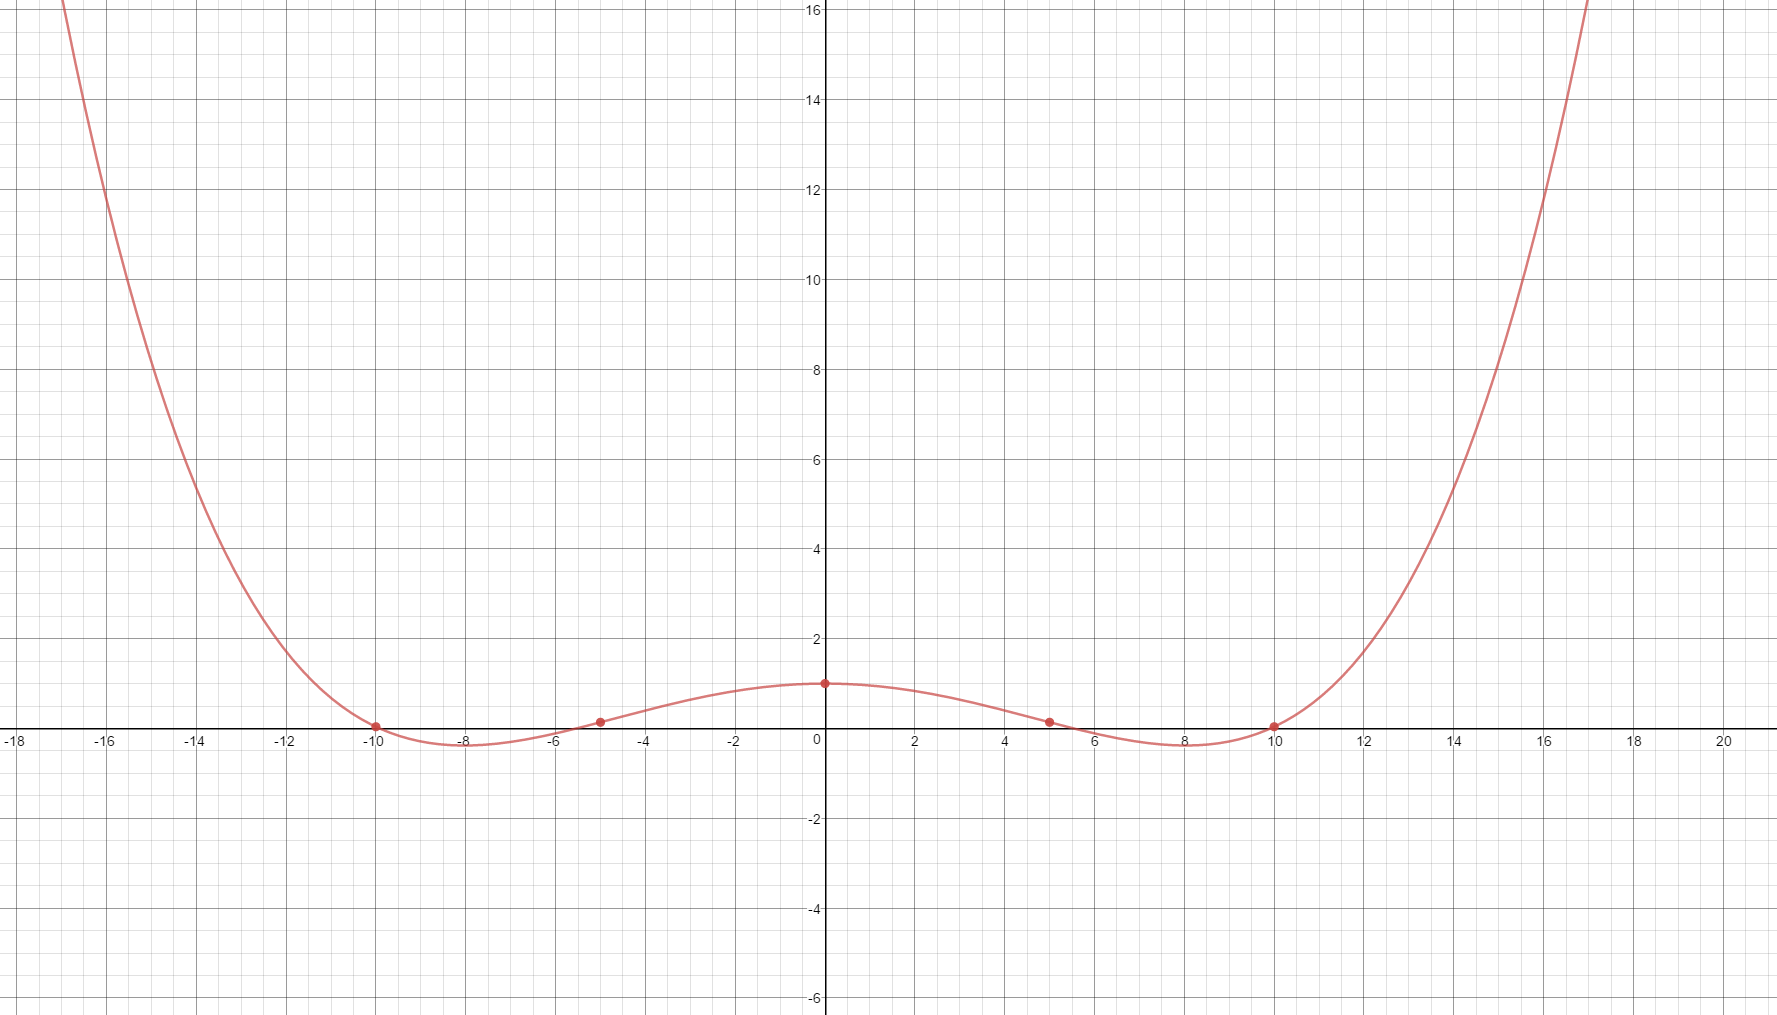
\includegraphics[scale=0.18]{img/1_4.png}
\end{figure}
Y la grafica de $f(x) - P_0(x)$:
\begin{figure}[H]
	\centering
	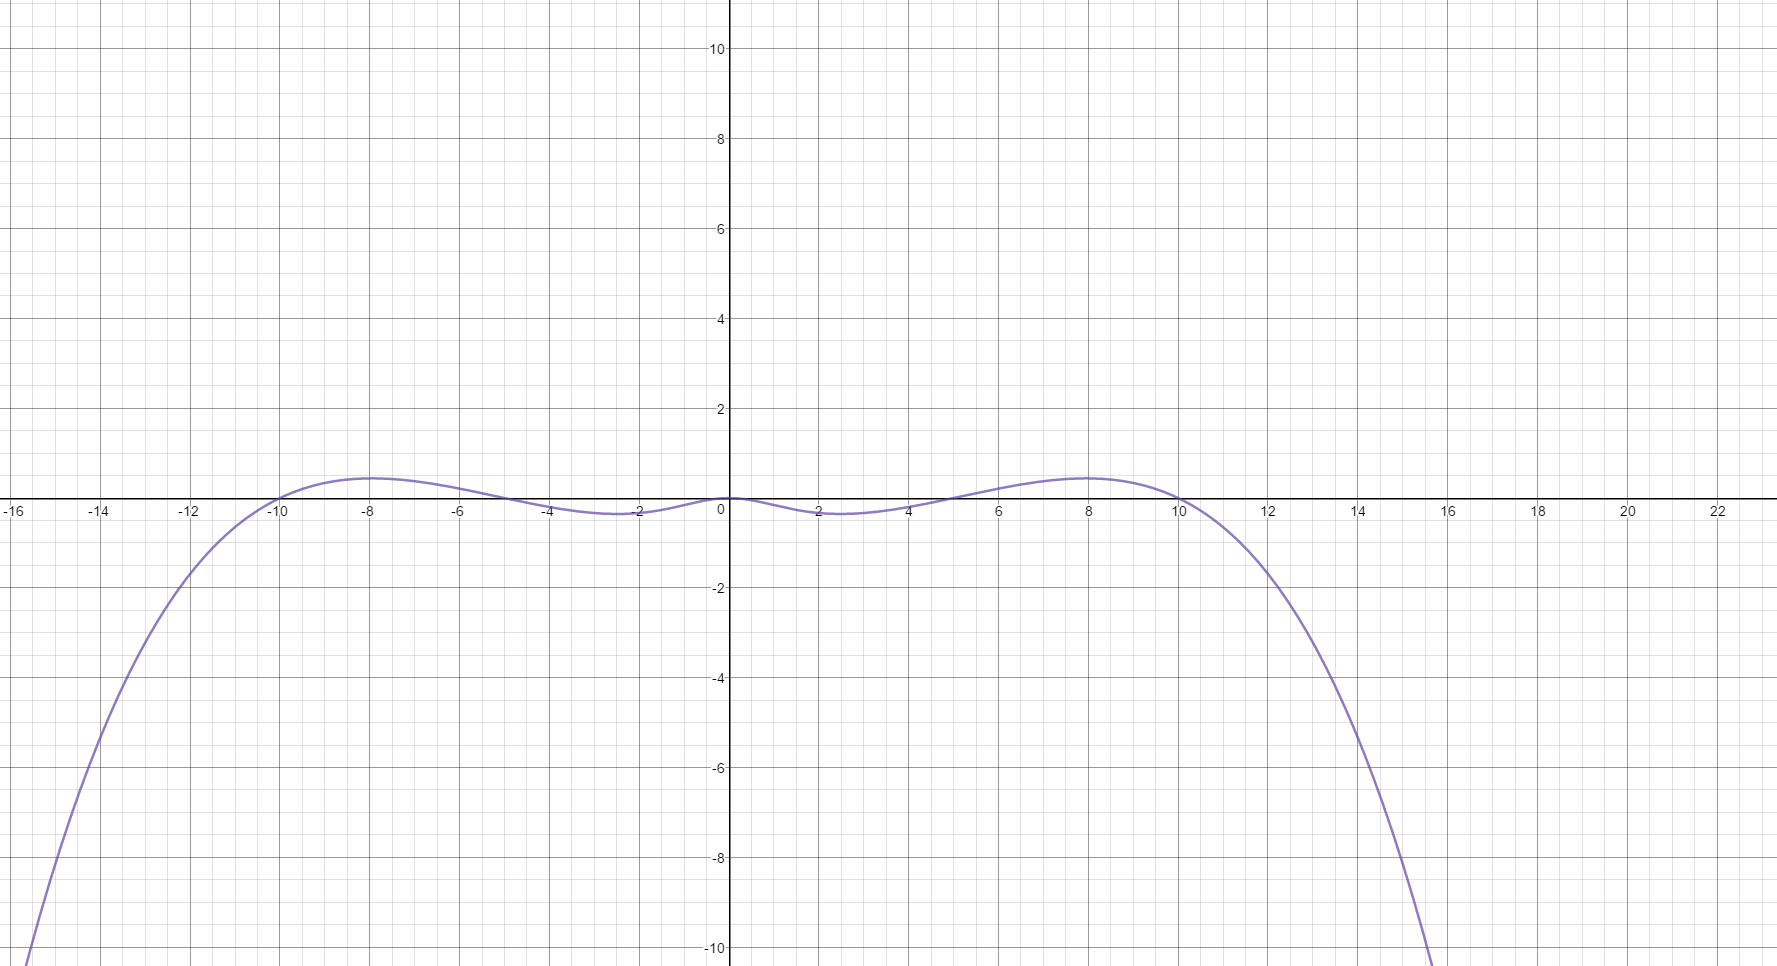
\includegraphics[scale=0.18]{img/1_4dif.png}
\end{figure}

Para $n = 7$ se obtiene el siguiente polinomio:
\begin{dmath}
P_1(x) = 0.03846154 +0.01198357 * (x +10.00000000 ) +0.00440345 * (x +10.00000000 ) * (x +7.14285714 ) +0.00218166 * (x +10.00000000 ) * (x +7.14285714 ) * (x +4.28571429 ) -0.00072895 * (x +10.00000000 ) * (x +7.14285714 ) * (x +4.28571429 ) * (x +1.42857143 ) +0.00008869 * (x +10.00000000 ) * (x +7.14285714 ) * (x +4.28571429 ) * (x +1.42857143 ) * (x -1.42857143 ) -0.00000517 * (x +10.00000000 ) * (x +7.14285714 ) * (x +4.28571429 ) * (x +1.42857143 ) * (x -1.42857143 ) * (x -4.28571429 ) +0.00000000 * (x +10.00000000 ) * (x +7.14285714 ) * (x +4.28571429 ) * (x +1.42857143 ) * (x -1.42857143 ) * (x -4.28571429 ) * (x -7.14285714 )
\end{dmath}
La grafica de $P_1(x)$:
\begin{figure}[H]
	\centering
	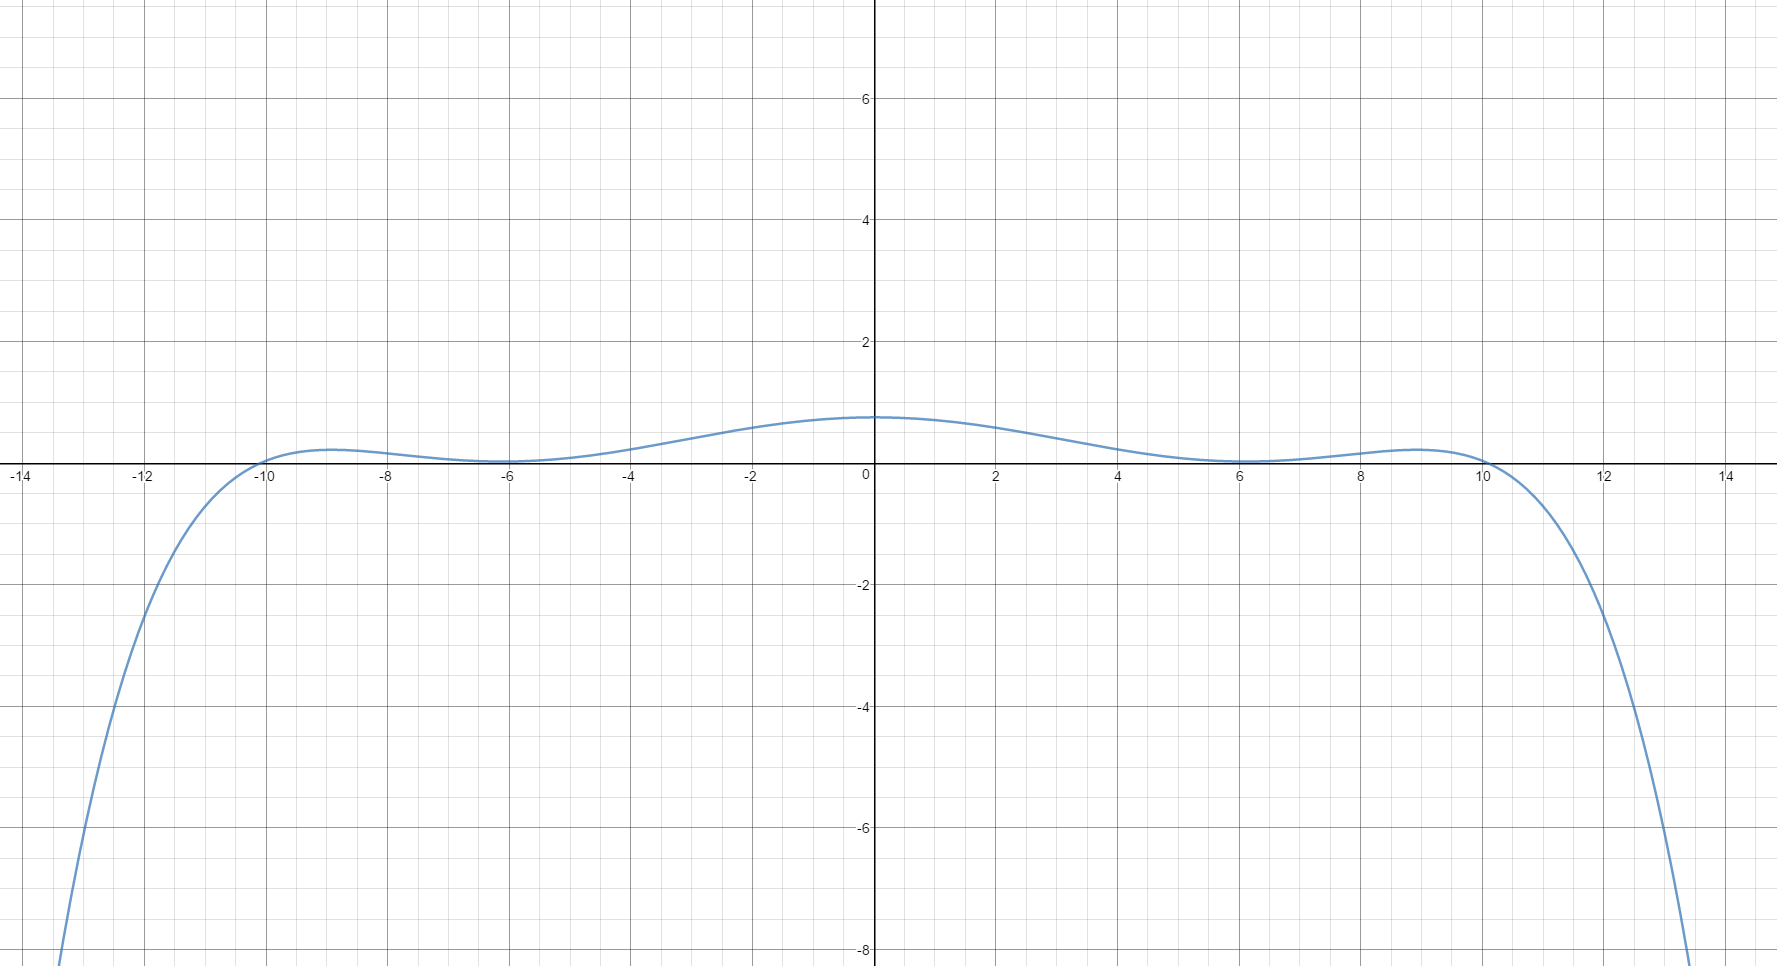
\includegraphics[scale=0.18]{img/1_7.png}
\end{figure}
Y la grafica de $f(x) - P_1(x)$:
\begin{figure}[H]
	\centering
	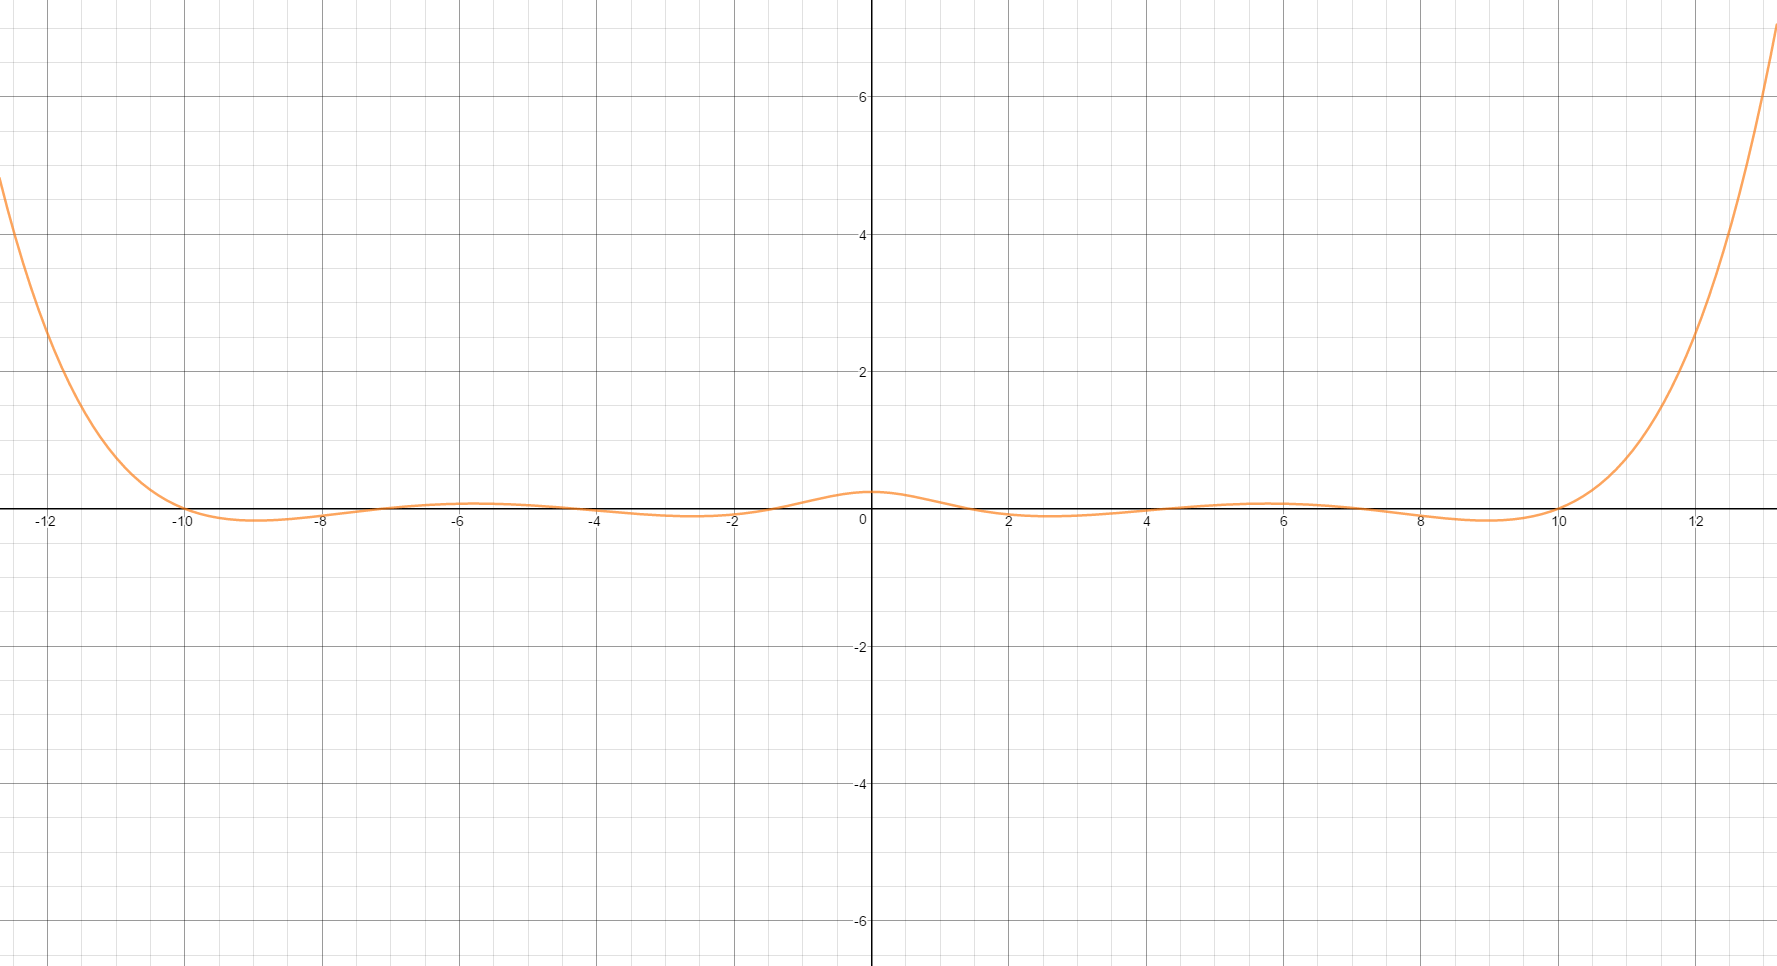
\includegraphics[scale=0.18]{img/1_7dif.png}
\end{figure}

Para $n = 10$ se obtiene el siguiente polinomio:
\begin{dmath}
P_2(x) = 0.03846154 +0.01018100 * (x +10.00000000 ) +0.00260181 * (x +10.00000000 ) * (x +8.00000000 ) +0.00079186 * (x +10.00000000 ) * (x +8.00000000 ) * (x +6.00000000 ) +0.00026867 * (x +10.00000000 ) * (x +8.00000000 ) * (x +6.00000000 ) * (x +4.00000000 ) -0.00006363 * (x +10.00000000 ) * (x +8.00000000 ) * (x +6.00000000 ) * (x +4.00000000 ) * (x +2.00000000 ) -0.00001768 * (x +10.00000000 ) * (x +8.00000000 ) * (x +6.00000000 ) * (x +4.00000000 ) * (x +2.00000000 ) * (x -0.00000000 ) +0.00000848 * (x +10.00000000 ) * (x +8.00000000 ) * (x +6.00000000 ) * (x +4.00000000 ) * (x +2.00000000 ) * (x -0.00000000 ) * (x -2.00000000 ) -0.00000168 * (x +10.00000000 ) * (x +8.00000000 ) * (x +6.00000000 ) * (x +4.00000000 ) * (x +2.00000000 ) * (x -0.00000000 ) * (x -2.00000000 ) * (x -4.00000000 ) +0.00000022 * (x +10.00000000 ) * (x +8.00000000 ) * (x +6.00000000 ) * (x +4.00000000 ) * (x +2.00000000 ) * (x -0.00000000 ) * (x -2.00000000 ) * (x -4.00000000 ) * (x -6.00000000 ) -0.00000002 * (x +10.00000000 ) * (x +8.00000000 ) * (x +6.00000000 ) * (x +4.00000000 ) * (x +2.00000000 ) * (x -0.00000000 ) * (x -2.00000000 ) * (x -4.00000000 ) * (x -6.00000000 ) * (x -8.00000000 )
\end{dmath}
La grafica de $P_2(x)$:
\begin{figure}[H]
	\centering
	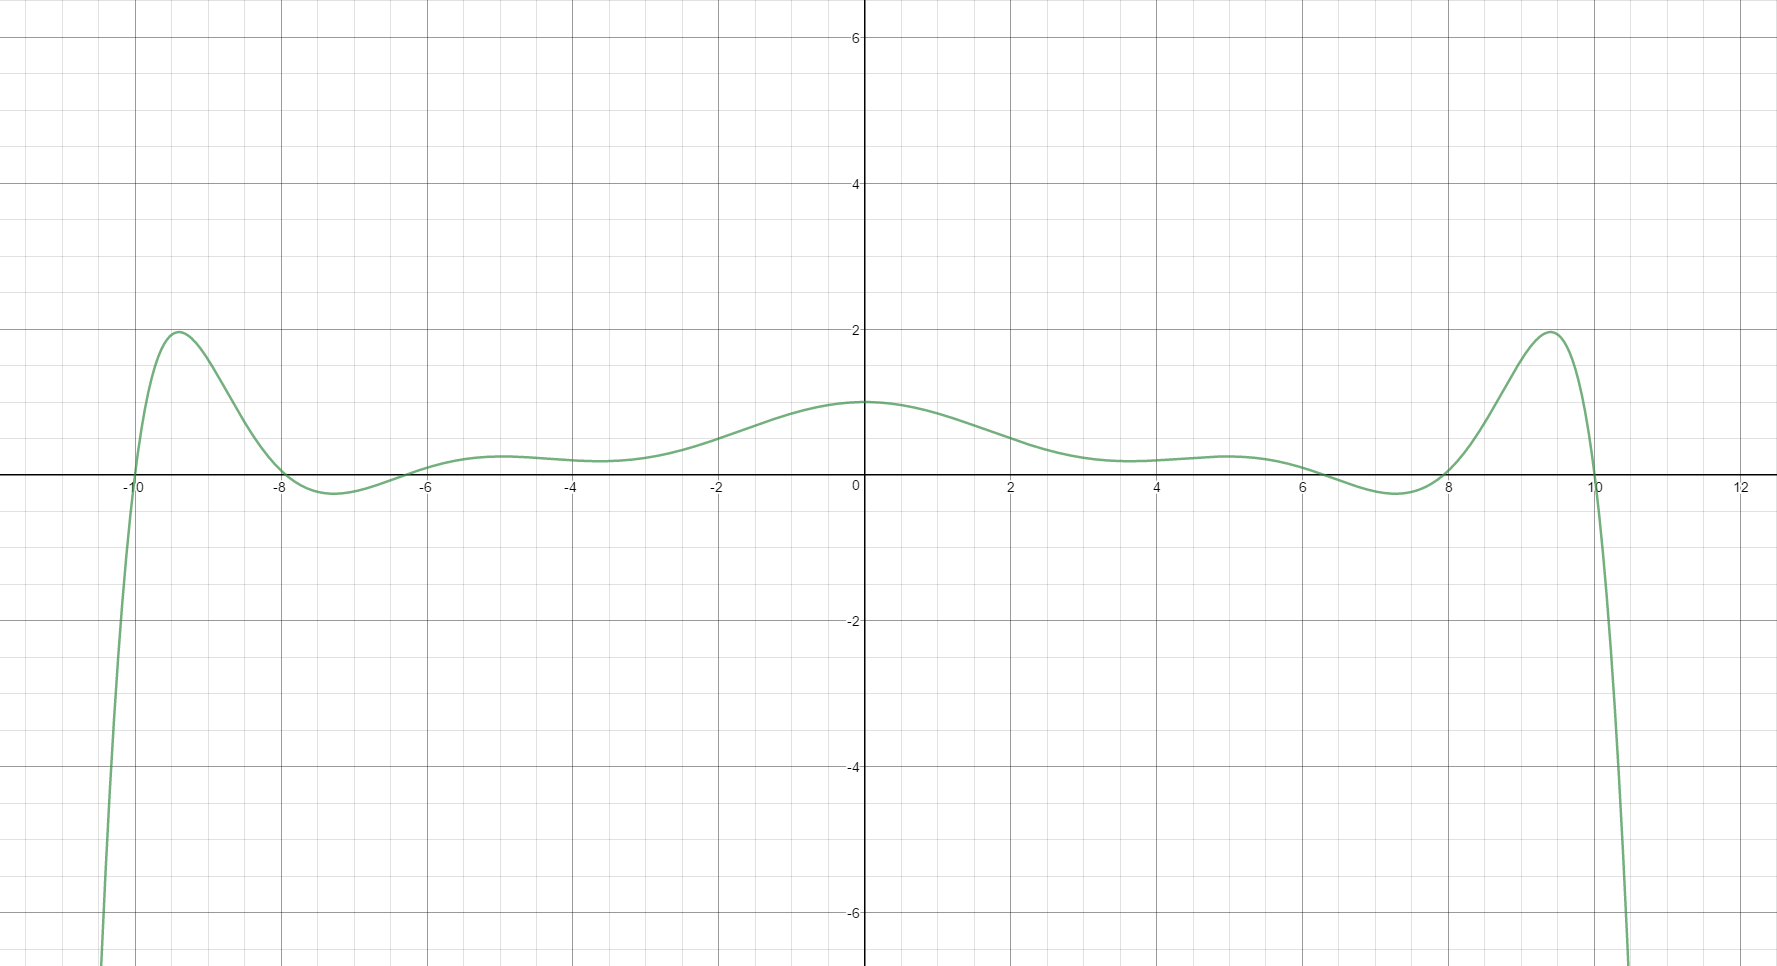
\includegraphics[scale=0.18]{img/1_10.png}
\end{figure}
Y la grafica de $f(x) - P_2(x)$:
\begin{figure}[H]
	\centering
	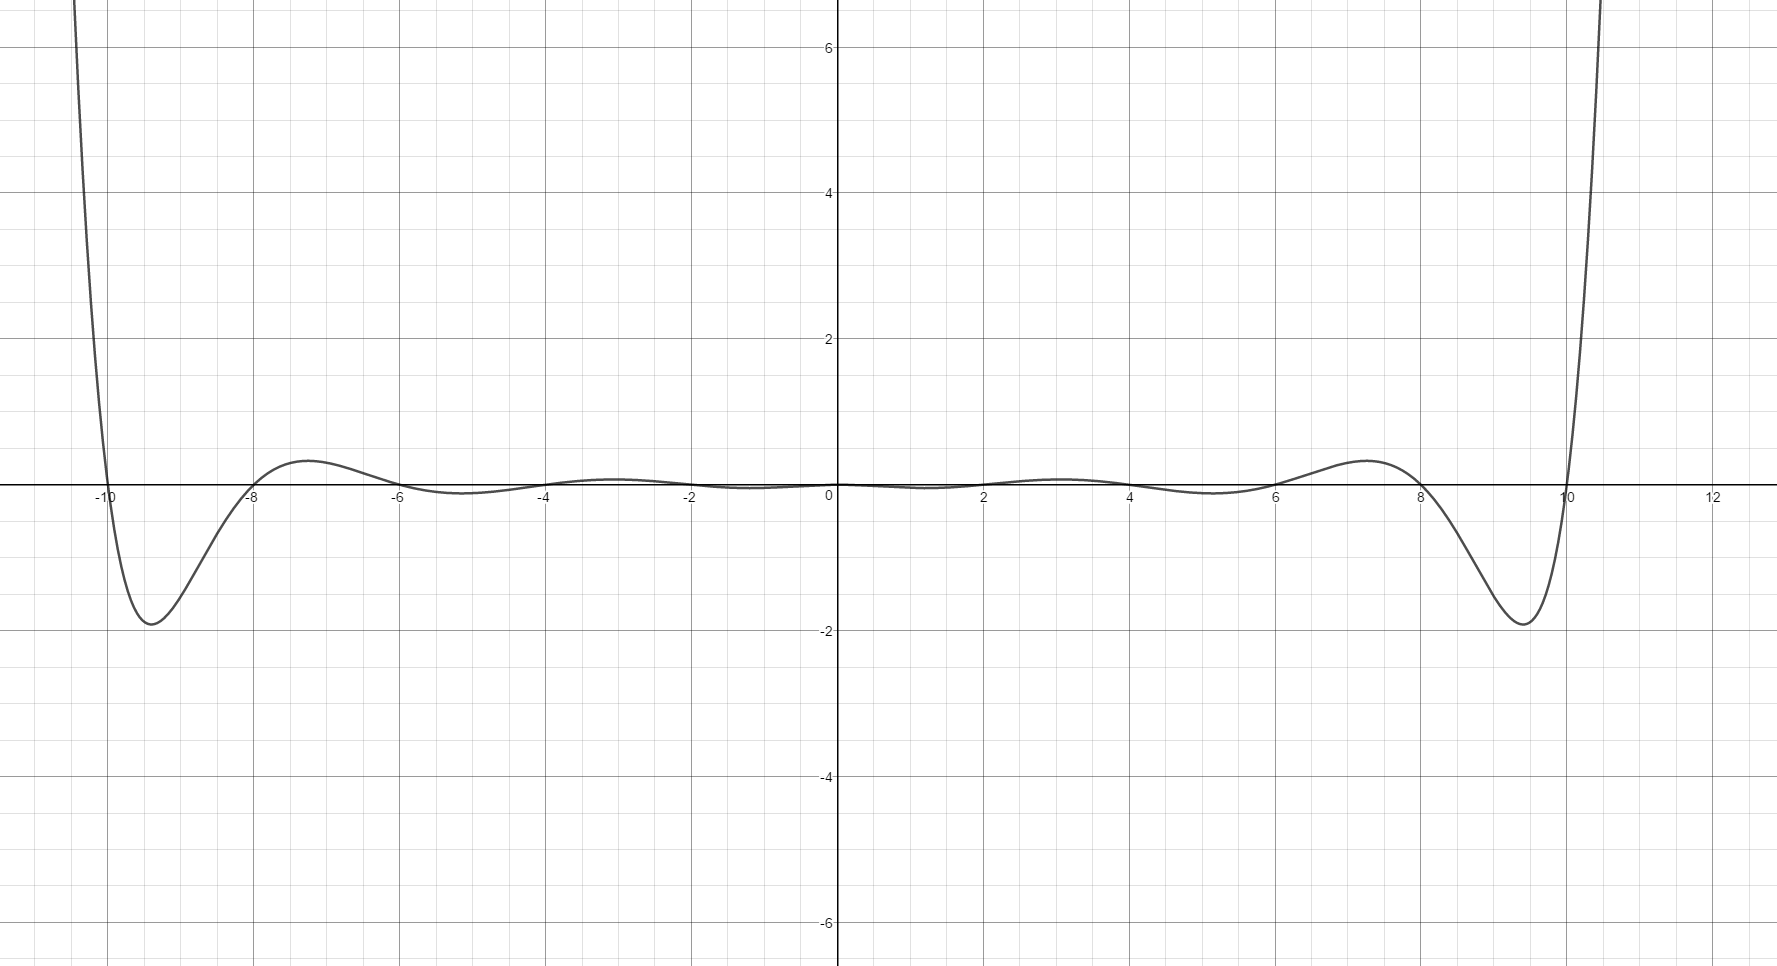
\includegraphics[scale=0.18]{img/1_10dif.png}
\end{figure}

Para ver cualquiera de estas gráficas con mas detalle, acceder al siguiente enlace \url{https://www.desmos.com/calculator/sqria4dpmp}